\documentclass{article}

\usepackage{amsmath}
\usepackage{amssymb}
\usepackage{csvsimple}
\usepackage{pgfplots}

\newcommand{\censuspicture}[1]{
\paragraph{}
\begin{tikzpicture}
		\begin{axis}[ xtick = {1900, 1920, ..., 2010},
				ytick = {50, 100, ..., 300},
				/pgf/number format/1000 sep={},
				xlabel={Year},
				ylabel={Population (Millions)},
				title={US Census Data}]
		\addplot table [x=year, y=Mpeople, col sep = comma]{#1};
	\end{axis}
\end{tikzpicture}
}

\newcommand{\modelpicture}[2]{
\paragraph{}
\begin{tikzpicture}
		\begin{axis}[ xtick = {1900, 1920, ..., 2010},
				ytick = {50, 100, ..., 300},
				/pgf/number format/1000 sep={},
				xlabel={Year},
				ylabel={Population (Millions)},
				title={US Census Data},
				legend pos=south east]
			\addplot table [x=year, y=Mpeople, col sep = comma]{#1};
			\addlegendentry{data};
			\addplot[color=red, mark=""] table [x=year, y=MPeople, col sep= comma]{#2};
			\addlegendentry{model};
	\end{axis}
\end{tikzpicture}
}
\begin{document}

\section{Outliers}

The total population of the US, as determined extremely precisely
	by the US census, is given below:

\censuspicture{data/census.csv}

\paragraph{}
In this problem, we modify the population in 1950 from 150.697 million 
	to 50.697 million, as if we forgot to type in the one when entering
	the data.  It now looks like this:

\censuspicture{data/modified-census.csv}

\paragraph{}
We try to answer the question:
Which of the models are the most and least affected by this outlier?
A model which handles the outlier well might ignore
	it and try to fit the rest of the data,
	or it might alert the user that something
	might be wrong with the data.
Alerting the user makes good sense in this case,
	especially since the ``story'' behind this outlier is from data
	entry error.
Models which handle this kind of an outlier poorly are ones for which
	the presence of an outlier significantly changes their fit, and
	makes their lines leave the data and try to find some middle
	ground.
This is not the desired behavior.

\paragraph{}
The models we are going to evaluate are:

\begin{enumerate}
\item Polynomial of degrees 1 to 4
\item PCHIP
\item Spline
\item Exponential
\end{enumerate}

\subsection{Polynomial Models}

\subsubsection{Linear Models}

We can try to fit a linear model with least squares.
First, to the original data:

\modelpicture{data/census.csv}{data/degree-1-census-fit.csv}

It's clear from the graph that the linear model isn't a good fit.
Next, to the outlier data:

\modelpicture{data/modified-census.csv}{data/degree-1-modified-census-fit.csv}

The model appears relatively resilient to the outlier.

The model moves slightly downwards, but the effect isn't extremely
	significant, and the outlier decreases the model's prediction
	for 2020 by only a few million people.

\subsubsection{Quadratic Models}

We can try to fit a quadratic model with least squares.
First, to the original data:

\modelpicture{data/census.csv}{data/degree-2-census-fit.csv}

The model fits the data quite well, 
Next, to the outlier data:

\modelpicture{data/modified-census.csv}{data/degree-2-modified-census-fit.csv}

The outlier seems to have a large effect.
The model is off the data for most of the way, and its
	predictions don't seem to make sense anymore.
The quadratic model seems to be somewhat sensitive to outliers.

\subsubsection{Cubic Models}

We can try to fit a cubic model with least squares.
First, to the original data fit to a cubic model:

\modelpicture{data/census.csv}{data/degree-3-census-fit.csv}

Note a very good correspondence with the data.
Next, to the outlier data:

\modelpicture{data/modified-census.csv}{data/degree-3-modified-census-fit.csv}

The model doesn't fit the data well here.
However, it's interesting to note that the model's predictions
	seem to be fairly accurate, and aren't far off from the
	original dataset.

\subsubsection{Conclusion}

Polynomial Models seem to have different behavior as
	the degree of the polynomials increases.
The higher degree the polynomials go, the worse the behavior
	near outliers will be.
However, the higher degree the polynomials go, the less the 
	outliers affect the predictions of the dataset for the 
	future.

\subsection{PCHIP}

PCHIP stands for Piecewise Cubic Hermite Interpolating Polynomial.
This method of interpolation attempts to make a piecewise polynomial
	which interpolates each data point.
Below is the PCHIP for the data with no outlier:

\modelpicture{data/census.csv}{data/pchip-census-fit.csv}

And the PCHIP for the data with the outlier:

\modelpicture{data/modified-census.csv}{data/pchip-modified-census-fit.csv}

The outlier hardle affects the prediction for 2020 at all.
However, the model happily accomodates the data point, moving down
	towards it.
This behavior is bad because the method doesn't recognize
	the data point as an outlier.

\subsection{Spline}

Cubic Splines are another interpolating method, similar to PCHIP.

\modelpicture{data/census.csv}{data/spline-census-fit.csv}

We see that the splines closely track the data, just as before.

\modelpicture{data/modified-census.csv}{data/spline-modified-census-fit.csv}

When the outlier is introduced, however, the splines have some 
	``overshoot'' near the outlier.
The region in which the outlier distorts the model, compared
	to the true data, is much larger.

The predictions are the same.

\subsection{Exponential Models}

We can make an exponential model by taking the log of both axes and
	then fitting with a linear model.
We might expect the linear model to be tolerant to outliers as before
	in ``log-space'', so I expect this model to be relatively tolerant.

\modelpicture{data/census.csv}{data/exponential-census-fit.csv}

This model actually doesn't fit the data as well as I anticipated.
I expected the exponential growth law to fit well, because it was 
	the first part of a population situation.
However, the model seems to be diverging from the data, especially
	towards the end.

\modelpicture{data/modified-census.csv}{data/exponential-modified-census-fit.csv}

The outlier pulls the model out significantly.

\subsection{Conclusion}

In summary, polynomial models are more resilient to outliers the lower
	degree they are, although higher degree polynomial models
	seem to be able to recover from outliers early in the data
	set to preserve their predictive value.
PCHIP and Spline models try to fit the data exactly, since they're 
	interpolating models.
The PCHIP does this better, because it minimizes the overshoot when 
	coming back to the normal data that we saw with the spline model.
Exponential Models seem to be easily distorted by outliers.

%%%%%%%%%%%%%%%%%%%%%%%%%%%%%%%%%%%%%%%%

\section{Rabbits and Foxes}

\subsection{Discussion of the model}

We have already justified the logistic model for a single species
	of animal.
How can we judge interactions between two species?

\subsubsection{Rabbit Dynamics}

Consider two coexisting populations of foxes and rabbits.
In the absence of foxes, the rabbits follow a logistic model
	for growth, with carrying capacity $K$ and growth rate $A$.
Once the foxes are introduced, predation occurs at a rate proportional
	to both the number of foxes and the number of rabbits.
If $R$ is the population of rabbits and $F$ is the population of 
	foxes, the differential equation describing rabbit population
	should be as follows, with $B$ a proportionality constant:

\begin{align}
	\frac{dR}{dt} & = A R \left( 1 - \frac{R}{K} \right) - B R F
\end{align}

\subsubsection{Foxes in Isolation}

Since we have introduced a new variable $F$, representing the number
	of foxes, we now need to determine its dynamics.
Suppose that in the absense of rabbits, the foxes die of starvation
	and other natural causes at a rate $C$, and proportional to their
	population.
This means that in the absence of rabbits, we would expect the foxes
	to die off exponentially.

This model is very simple and somewhat flawed, because past a certain
	time without food, we wouldn't expect any foxes to be alive,
	but the exponential model never decreases exactly to zero.
Therefore this model won't be predictive when there are very few
	foxes.

\subsubsection{Fox Predation}

Suppose that from predating the rabbits, the foxes gain in population
	at a rate proportional to their population and the rabbits' population.
This can be interpreted as the equilibrium limit of the independent
	chances of any given fox catching any other rabbit.
This model obviously ignores many factors, but it's the simplest which
	captures the essence of predation.

The if $D$ is the predation proportionality constant, then the differential
	equation encoding the dynamics of the fox population
	is as follows:

\begin{align}
	\frac{dF}{dt} & = \left( D R - C \right) F
\end{align}

\subsection{Equilibria}

The full system of coupled differential equations is as follows:

\begin{align}
	\frac{dR}{dt} & = A R \left( 1 - \frac{R}{K} \right) - B R F\\
	\frac{dF}{dt} & = \left( D R - C \right) F
\end{align}

If the system is in equlibrium, then $\frac{dF}{dt} = 0$.
Thus, either $R = \frac{C}{D}$ or $F = 0$.

If the system is in equilibrium, then $\frac{dR}{dt} = 0$.
Suppose $F = 0$.
Then, $A R \left( 1 - \frac{R}{K} \right) = 0$, and thus
	either $R = 0$ or $R = K$.

Suppose $R = \frac{C}{D}$.
Then, $A \frac{C}{D} \left( 1 - \frac{C}{D} \frac{1}{K} \right) 
	- B \frac{C}{D} F = 0$.
Therefore, $F = \frac{A}{B} \left( 1 - \frac{C}{D} \frac{1}{K} \right)$.

We summarize all of the equilibrium points in a table.

\paragraph{}
\begin{tabular}{|l|l|}
\hline
$R$ & $F$ \\
\hline
$0$ & $0$ \\
\hline
$K$ & $0$ \\
\hline
$\frac{C}{D}$ & $\frac{A}{B} \left( 1 - \frac{C}{D} \frac{1}{K} \right)$ \\
\hline
\end{tabular}

\paragraph{}
To help visualize the stable point for which the populations 
	of both rabbits and foxes are nonzero, I plotted the following
	diagram.
The position of the stable point is determined by the position
	of $\frac{C}{D}$ on the foxes axis, where $K = 1$.
We see immediately that this stable point isn't even in the 
	state space when $\frac{C}{D} > K$.


\paragraph{}
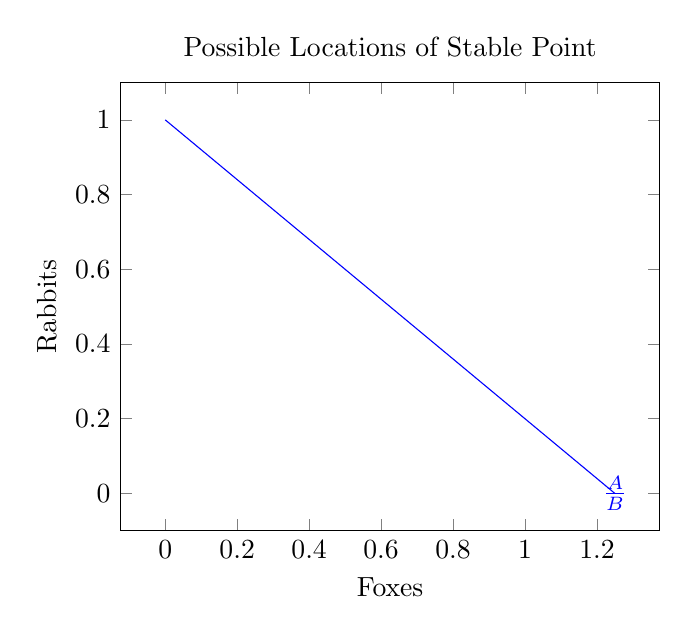
\begin{tikzpicture}
	\begin{axis}[ xlabel=Foxes
				, ylabel=Rabbits 
				, title=Possible Locations of Stable Point]
				\addplot[color=blue, mark=""] coordinates {
			(0,1)
			(1.25,0)
	} node(endofline) {$\frac{A}{B}$};
	\end{axis}
\end{tikzpicture}


\subsubsection{Which ones are additional?}

We are treating this model as a modification to a model
	in which the rabbits are described by an exponential
	growth model in the absence of foxes.
This corresponds to sending the carrying capacity to infinity.
Note that if the carrying capacity goes to infinity,
	then the second equilibrium point disappears,
	and the $\frac{1}{K}$ in the third one becomes zero.
The term with $\frac{1}{K}$ represents the modification to this
	model from the finite carrying capacity of the rabbits.

\subsection{Stability of Equilibria}

To determine whether an equilibrium point is stable or unstable,
	we can treat the dynamics around the equilibrium point
	as a linear system, even if the overall dynamics are nonlinear.
This involves an object called the Jacobian.
The jacobian for this system of differential equations is:

\begin{align}
	J(R,F) & = \left[ 
		\begin{array}{cc} 
			\frac{\partial \left(\frac{dR}{dt}\right)}
				{\partial R}
		& 
			\frac{\partial \left(\frac{dF}{dt}\right)}
				{\partial R}
		\\
			\frac{\partial \left(\frac{dR}{dt}\right)}
				{\partial F}
		&
			\frac{\partial \left(\frac{dF}{dt}\right)}
				{\partial F}
		\\
		\end{array} \right]
	& = \left[ \begin{array}{cc}
			\left( A - B F \right) - 2 A \frac{R}{K}
		&
			- B R
		\\
			D F
		&
			D R - C
		\\
		\end{array} \right]
\end{align}

The stability in the neighborhood of each equilibrium
	point is given by the eigenvalues of each jacobian,
	evaluated at that point.

\paragraph{}
\begin{tabular}{l|l|l|l}
$R$ & $F$ & $\lambda_1$ & $\lambda_2$ \\
$0$ & $0$ & $A$ & $-C$ \\
$K$ & $0$ & $-A$ & $D \left( K - \frac{C}{D} \right)$ \\
$\frac{C}{D}$ & $\frac{A}{B} \left(1 - \frac{C}{D} \frac{1}{K} \right)$ 
	& $ \frac{A}{2} \frac{C}{D} \left( - \frac{1}{K}
		+ \sqrt{ \frac{1}{K^2} + \frac{4 B}{A}
			\left( \frac{1}{K} - \frac{D}{C} \right) } \right) $
	& $ \frac{A}{2} \frac{C}{D} \left( - \frac{1}{K}
		- \sqrt{ \frac{1}{K^2} + \frac{4 B}{A}
			\left( \frac{1}{K} - \frac{D}{C} \right) } \right) $ \\ 
\end{tabular}

\subsubsection{Stability of points on the ``Rabbit Axis''}

Zero will always be a saddle point, attractive from the foxes
	side, because foxes die with no rabbits,
	and repelling from the rabbits side, because without foxes
	rabbits grow logistically.
The rabbits' carrying capacity is sometimes stable, and sometimes
	unstable.
If $K > \frac{C}{D}$, then both eigenvalues are negative,
	and it is attracting from all sides.
However, if $K < \frac{C}{D}$, the rabbits' carrying capacity
	becomes a saddle, and it repels in the direction of more foxes.

\subsubsection{Stability of center point}

The center point is algebraically more tricky to deal with.
We can notice the $\frac{1}{K^2}$ term in the square root.
If the other term were zero, than in $\lambda_1$,
	the value of the square root would exactly cancel out
	the leading $- \frac{1}{K}$, and the eigenvalue would be $0$.
Therefore, if the other term within the square root is greater 
	than zero, then we would expect $\lambda_1$ to be positive,
	and if it is less than zero, we would expect $\lambda_1$
	to be negative.
The term in question is 
	$\frac{4 B}{A} \left( \frac{1}{K} - \frac{D}{C} \right)$.

If $K > \frac{C}{D}$, then the term is positive, and $\lambda_1$
	is positive, and therefore repelling.
This might be significant, but if we plug in the position for the
	stable point itself, we find that it is in fact not in
	the positive quadrant, and we can remove it from consideration.

The other eigenvalue is still negative, and therefore, if $K > \frac{C}{D}$,
	the internal stable point is a saddle.
If, however, $K < \frac{C}{D}$, then the term is negative,
	and the total value of $\lambda_1$ is thus negative.
Then the internal stable point is attractive.

Note that if $K = \frac{C}{D}$, then the two nonzero fixed points
	are actually on top of each other.

\subsubsection{Conclusion}

To sum up, when $K > \frac{C}{D}$, the foxes die out and the
	rabbits reach their carrying capacity.
However, if $K < \frac{C}{D}$, then the foxes survive
	and the rabbit-fox population reaches an equilibrium
	with $\frac{C}{D}$ rabbits and a nonzero amount of foxes.
For a predator species, the key factor for survival is the ratio
	between how much they can get from predation, $D$,
	and the rate at which they starve, $C$.
If they can push the ratio $\frac{C}{D}$ above the carrying capacity
	of a prey species, then they can safely predate them.
However, if they starve too fast, or derive too little nutrients
	from the prey, then they will die off.

\subsection{Phase Portraits}

This is the case where the carrying capacity $K$ is much greater than
	$\frac{C}{D}$.
The population periodically oscillates around a central point,
	which is an attracting center.

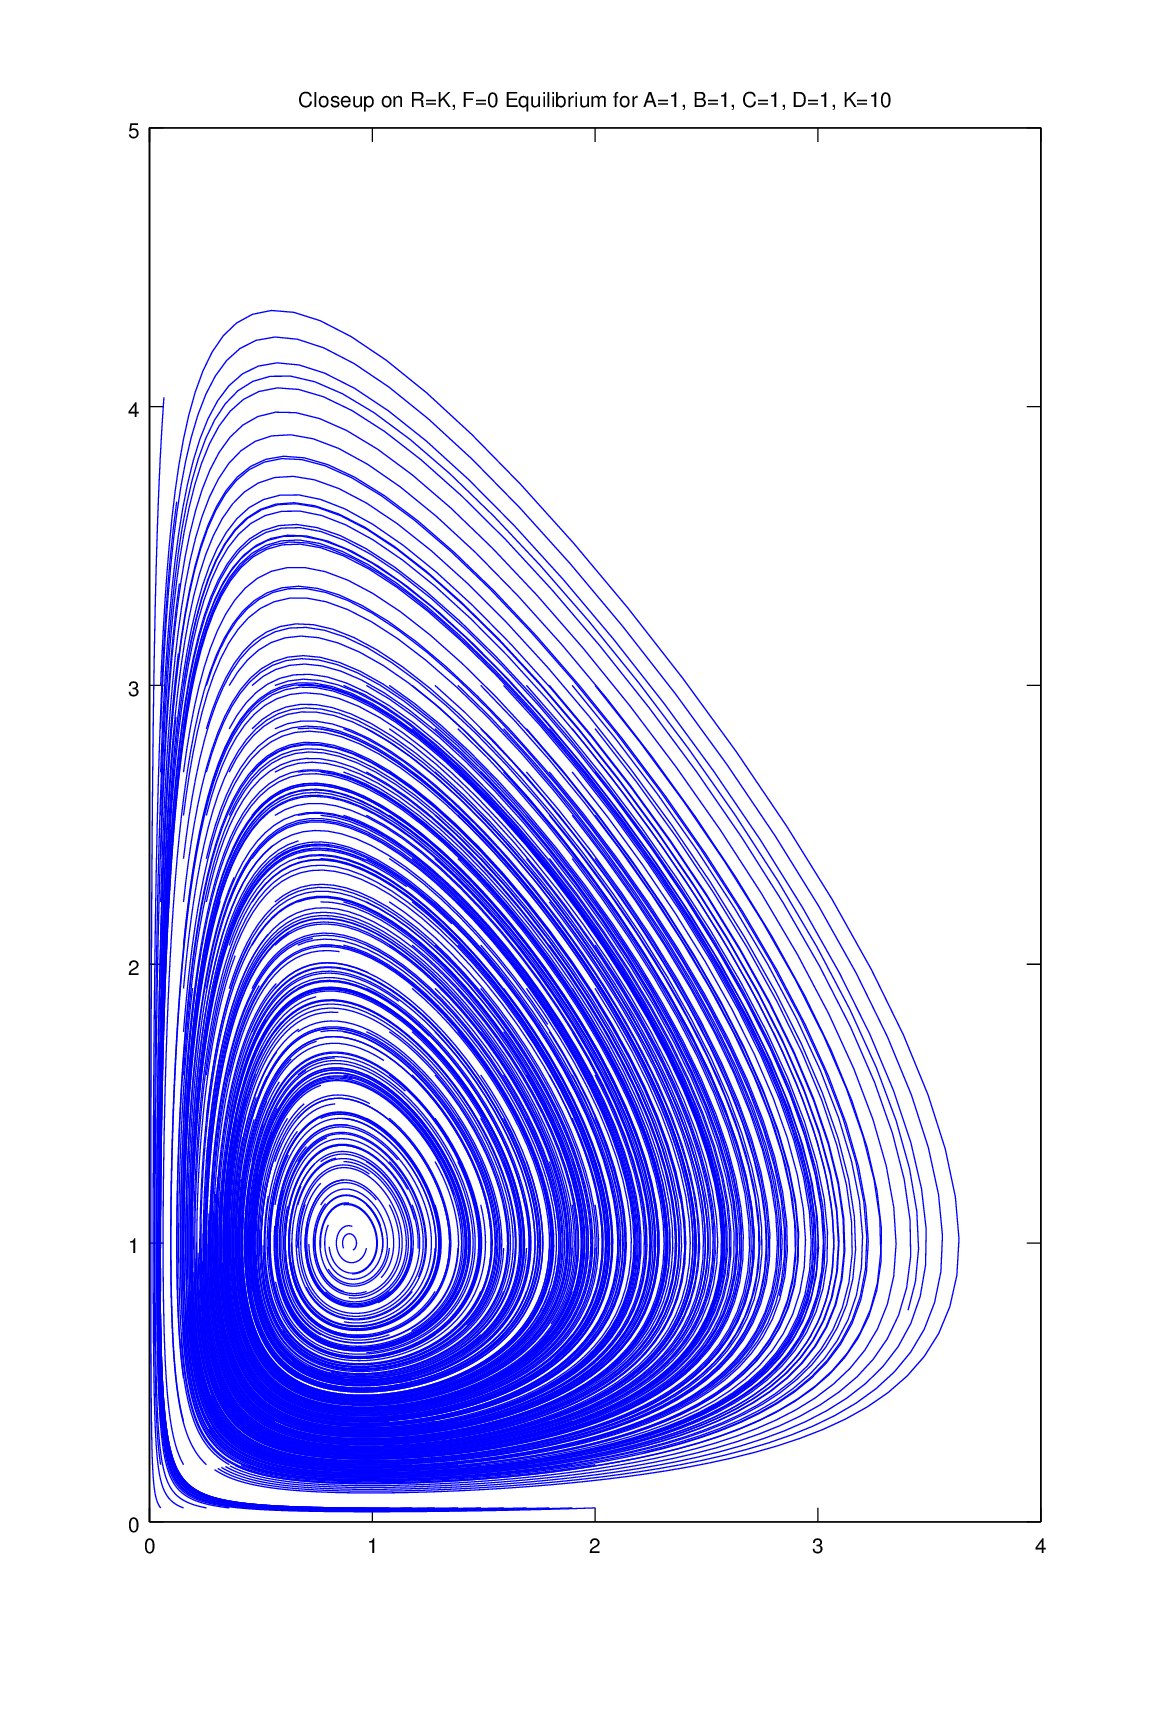
\includegraphics[width=\textwidth]{plots/phase-potrait.png}

As we bring $K$ down to just above $\frac{C}{D}$,
	the cycle stretches as it gets near $K$ on the 
	rabbits axis.

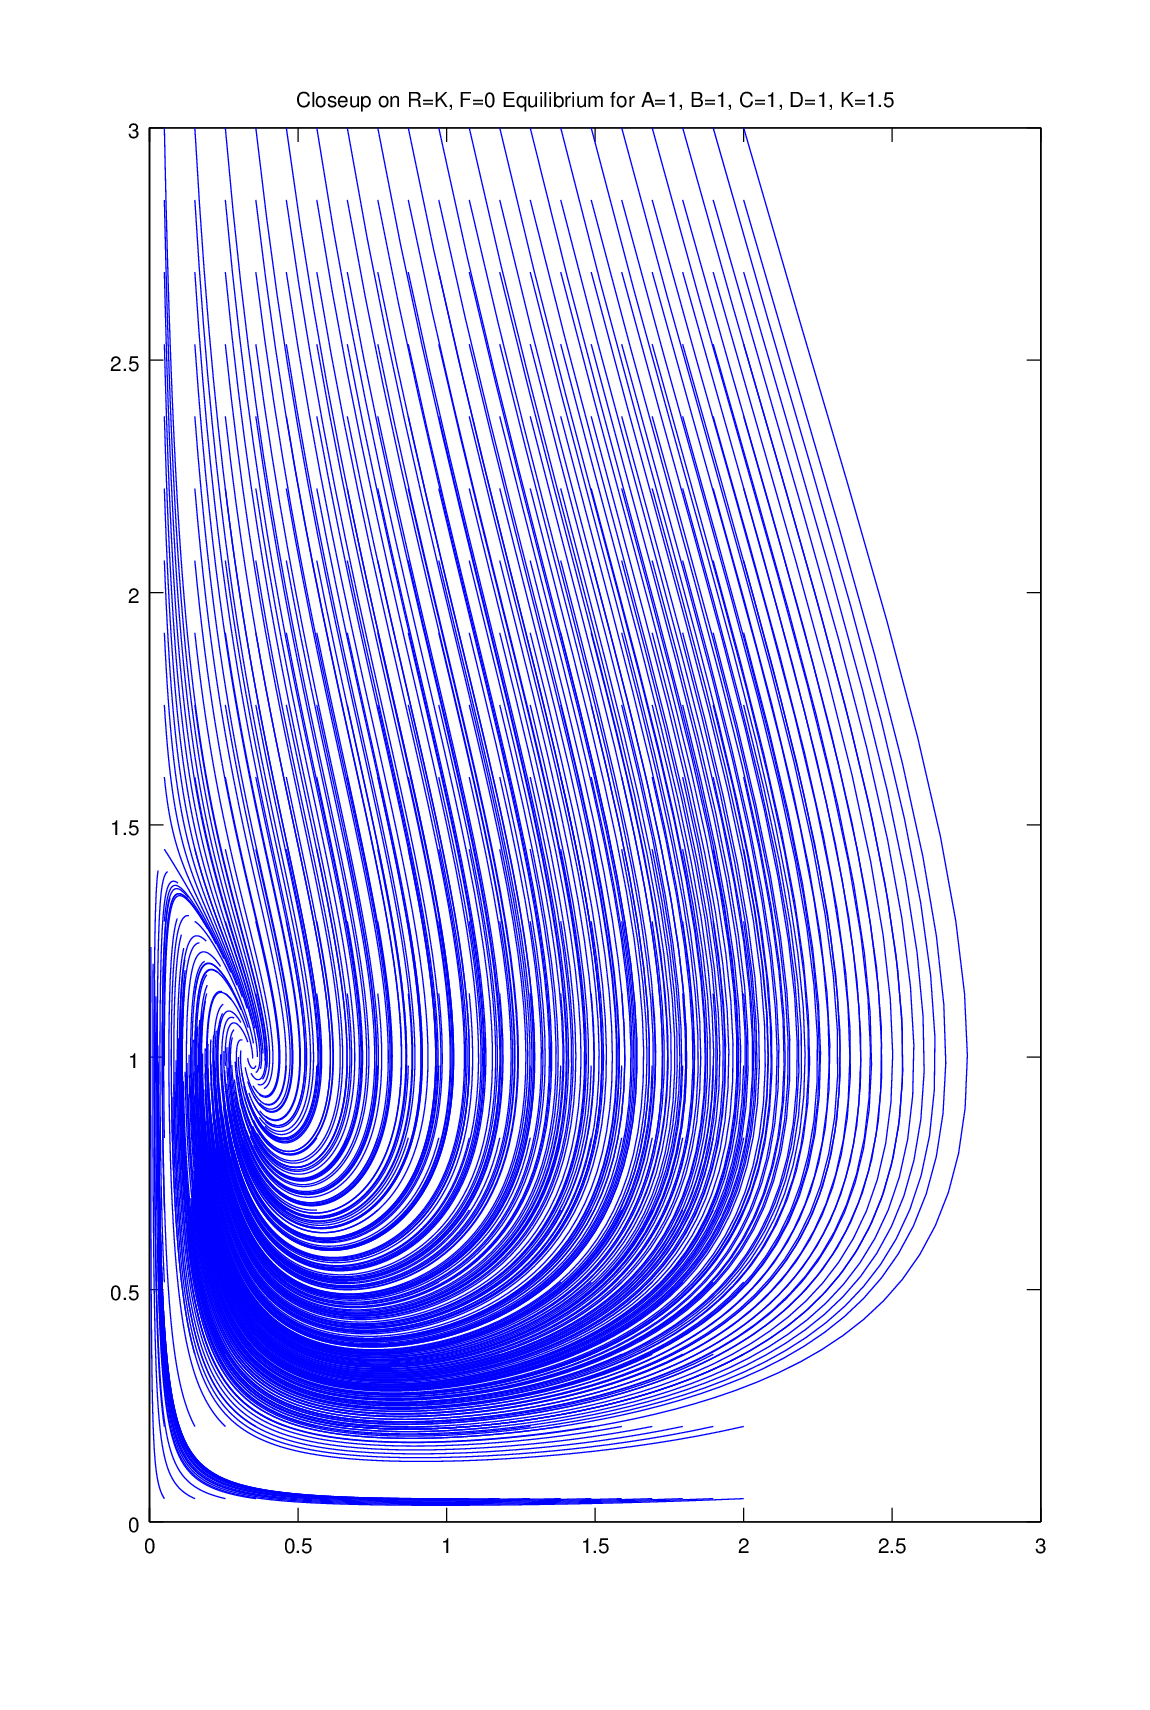
\includegraphics[width=\textwidth]{plots/phase-potrait-near-degenerate.png}

When $\frac{C}{D} = K$, the total field is attracted slowly.

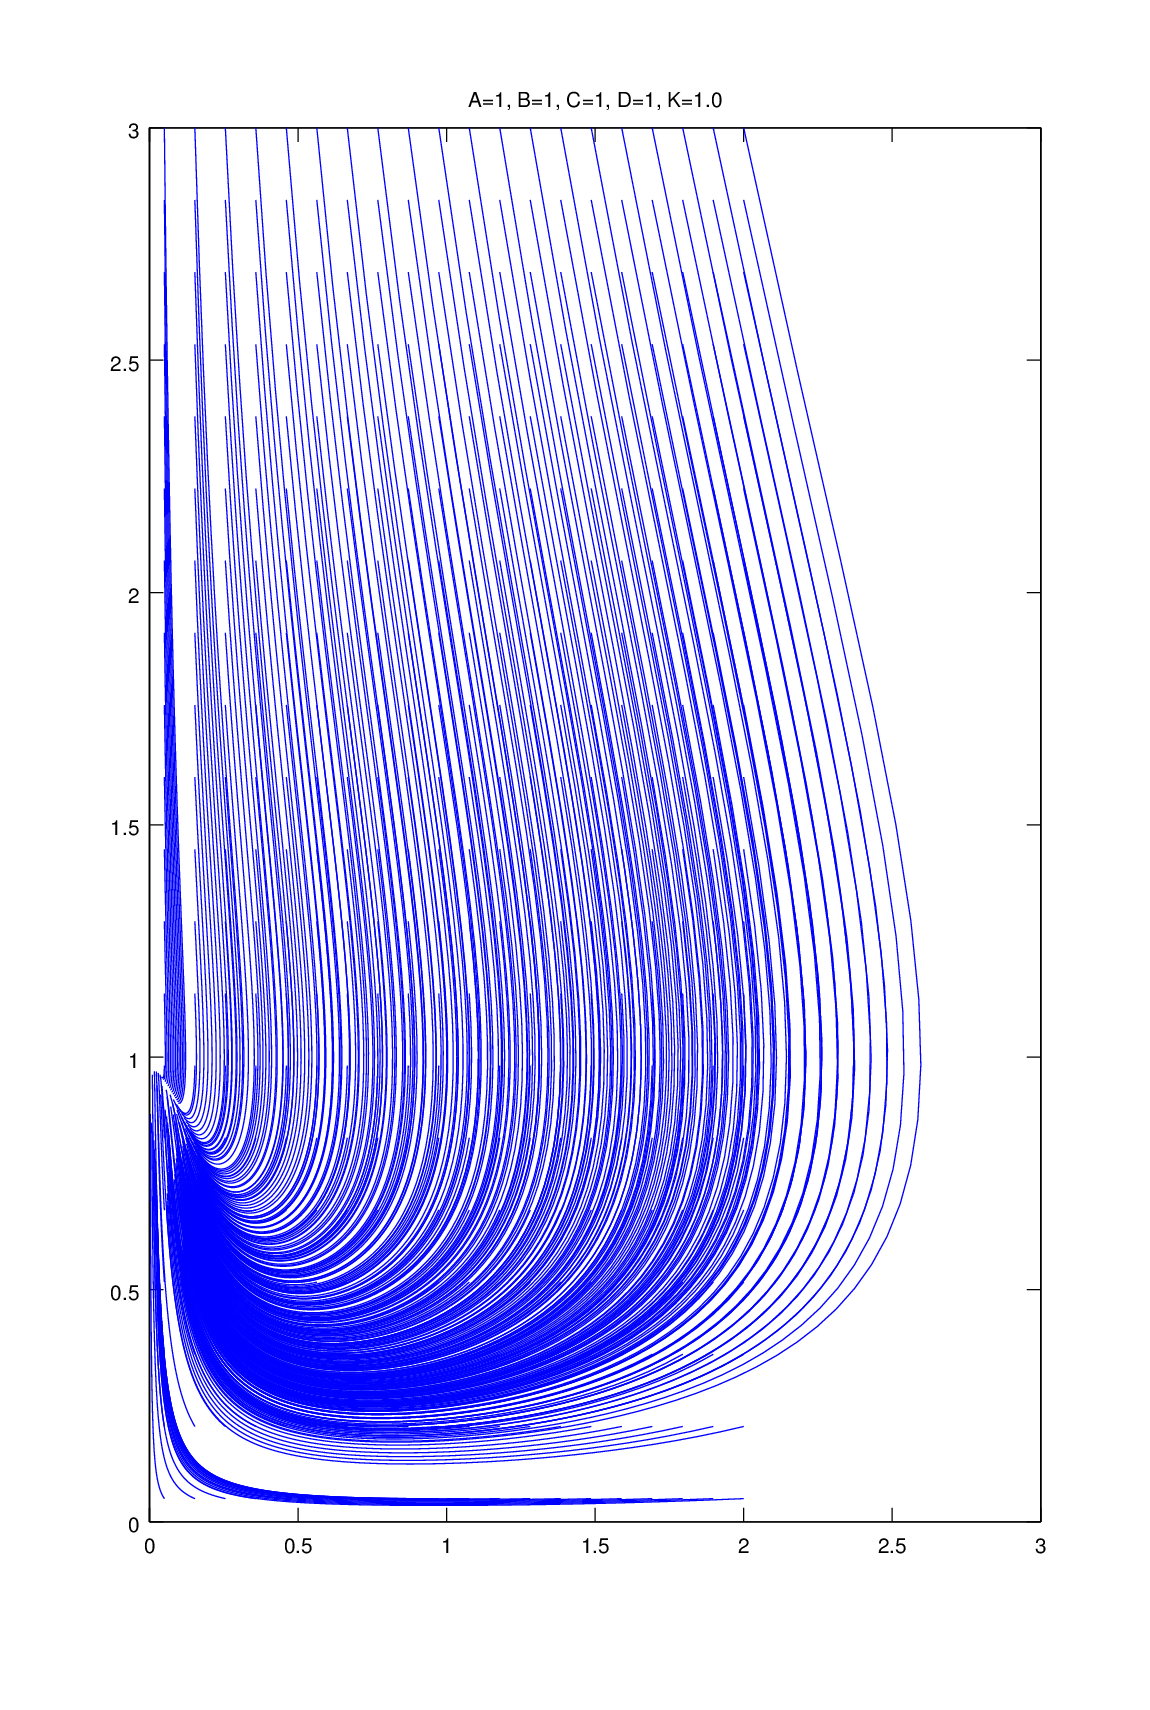
\includegraphics[width=\textwidth]{plots/phase-potrait-degenerate.png}

The whole state space is attracted more quickly to the only-rabbits
	state.

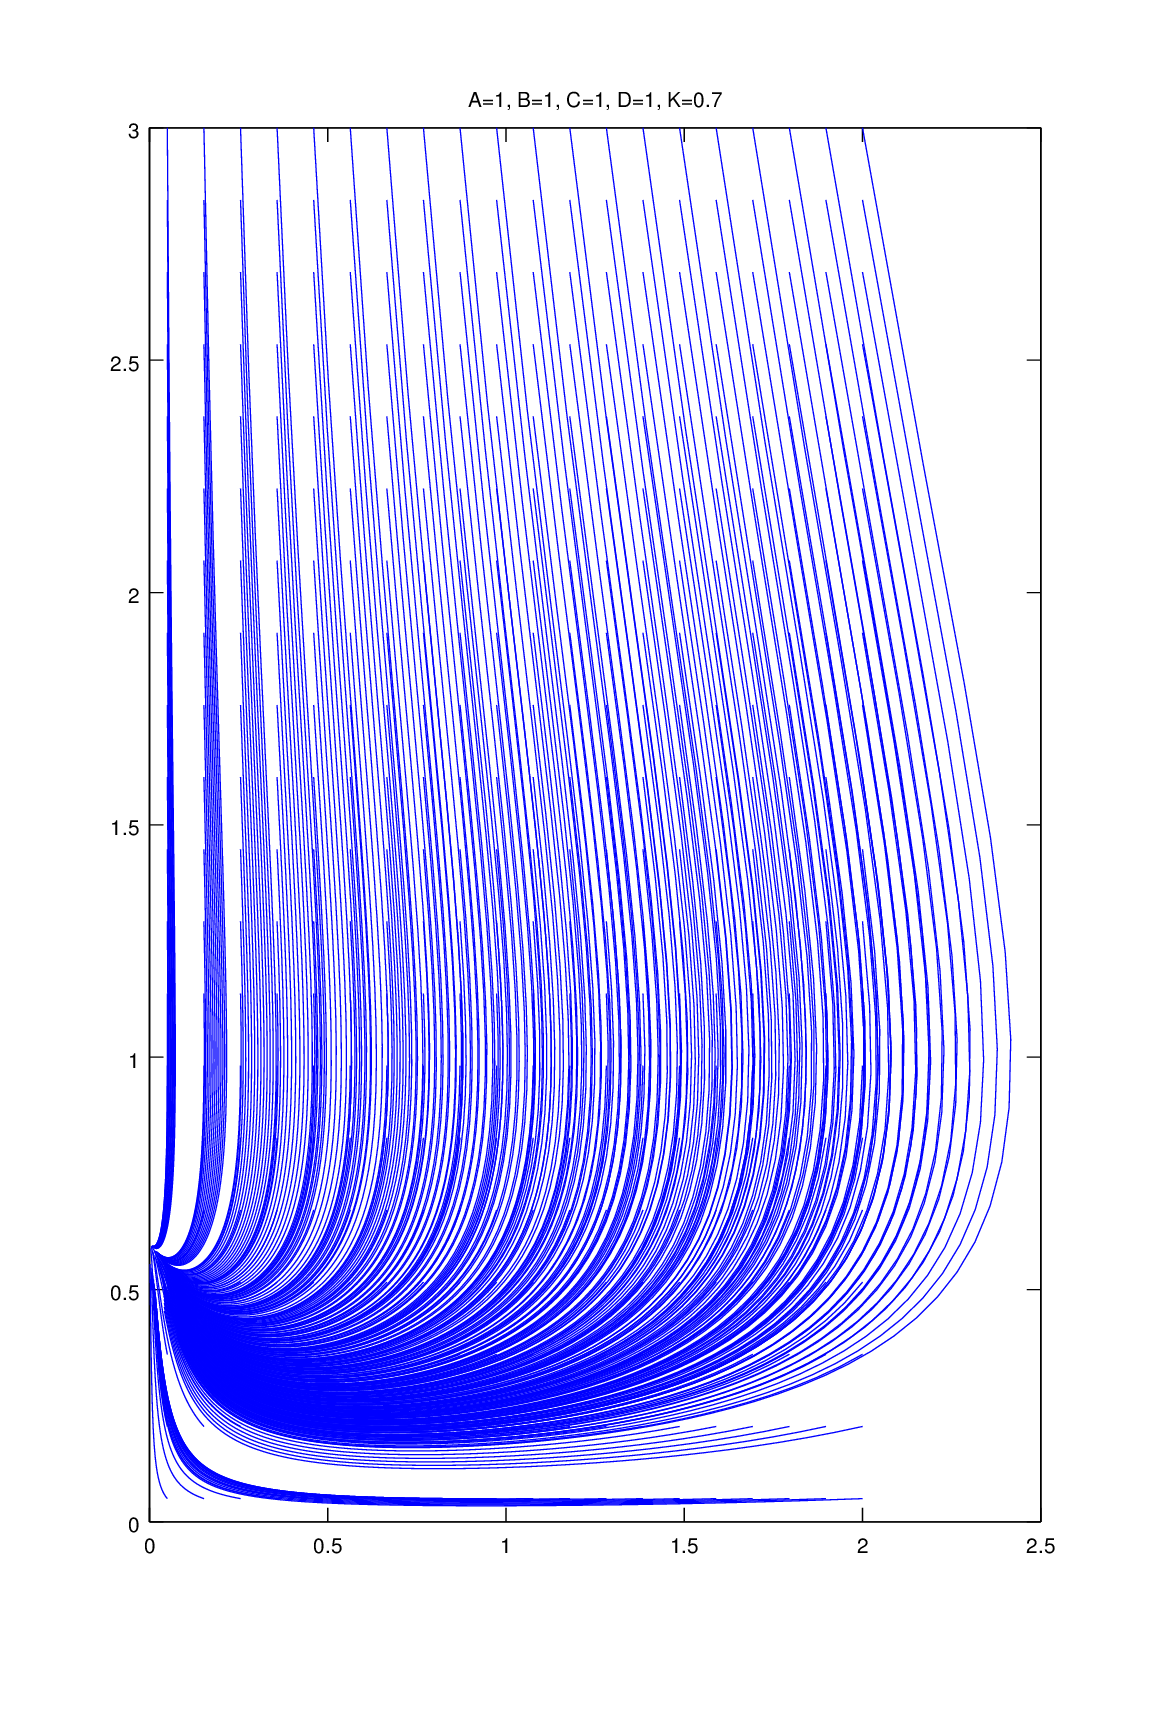
\includegraphics[width=\textwidth]{plots/phase-potrait-past-degenerate.png}

\end{document}
